\documentclass[12pt]{article}
\usepackage[left=0.5in, right=0.5in, top=0.5in, bottom=0.5in]{geometry}
\usepackage{ulem}
\usepackage{amsmath}
\usepackage{enumerate}
\usepackage{graphicx}
\usepackage[utf8x]{inputenc}
\usepackage{amsmath}
\graphicspath{ {images/} }

\begin{document}
\begin{flushleft}
Andy Liang

CSE 150 - Foundations of Computer Science: Honors

Professor Bender
\end{flushleft}
\medskip
\centerline{\uline{Homework 1B}}
\bigskip\bigskip

\noindent
\uline{Problem 4}
\\\textbf{Boolean algebra operations can be expressed as arithmetic operations mod 2. Let 1 be true, and 0 false.}
\begin{enumerate}[(a)]
\item \textbf{Show that A $\land$ B = (A $\cdot$ B mod 2).}
\item \textbf{What is $\neg A$?}
\item \textbf{What is A $\lor$ B?}
\end{enumerate}
\medskip
\uline{Response}
\begin{enumerate}[(a)]
\item 
\begin{tabular}{c|c|c}
A & B & $A \lor B$\\
\hline
T & T & T\\
T & F & F\\
F & T & F\\
F & F & F\\
\end{tabular}
\hspace{1in}
\begin{tabular}{c|c|c|c}
A & B & A $\cdot$ B & A $\cdot$ B mod 2\\
\hline
1 & 1 & 1 & 1\\
1 & 0 & 0 & 0\\
0 & 1 & 0 & 0\\
0 & 0 & 0 & 0\\
\end{tabular}
\medskip
\item $\neg A = (A + 1)$ mod 2
\vspace{0.1in}
\\*\begin{tabular}{c|c}
A & $\neg A$\\
\hline
T & F\\
F & T\\
\end{tabular}
\qquad\qquad
\begin{tabular}{c|c|c}
A & $A + 1$ & $(A + 1)$ mod 2\\
\hline
1 & 2 & 0\\
0 & 1 & 1\\
\end{tabular}
\medskip
\item $A \lor B = (((A+1) \cdot (B+1)$ + 1) mod 2)
\vspace{0.1in}
\\*\begin{tabular}{c|c|c}
A & B & $A \lor B$\\
\hline
T & T & T\\
T & F & T\\
F & T & T\\
F & F & F\\
\end{tabular}
\bigskip
\\*
\begin{tabular}{c|c|c|c|c|c|c}
A & B & A + 1 & B + 1 & (A + 1) $\cdot$ (B+1) & (A + 1) $\cdot$ (B+1) + 1 & ((A+1) $\cdot$ (B+1) + 1) mod 2\\
\hline
1 & 1 & 2 & 2 & 4 & 5 & 1\\
1 & 0 & 2 & 1 & 2 & 3 & 1\\
0 & 1 & 1 & 2 & 2 & 3 & 1\\
0 & 0 & 1 & 1 & 1 & 2 & 0\\
\end{tabular}
\end{enumerate}
\bigskip
\newpage
\noindent
\uline{Problem 5}
\\\textbf{Over lunch at the faculty club, n professors are expressing their concerns over their salaries. Each
professor wants to know how his/her salary compares to the average salary of the group, but no
professor wants to divulge any information about his/her salary to the other n - 1.}
\begin{enumerate}[(a)]
\item \textbf{Devise a scheme that allows the professors to compute the average of their salaries, while
preserving their privacy.
\\You may assume that all the professors will adhere to the rules of the protocol, although they
will try to extract as much information from the protocol as possible. You may also assume
that it is public knowledge that the professors' salaries together don't exceed \$1 trillion.}
\item \textbf{Now extend the protocol to be robust even when groups of professors collude. Specifically, if \textit{i} professors collude, naturally they can learn the average salary of the remaining n - \textit{i}. Your protocol should reveal no additional information.}
\end{enumerate}
\medskip

\noindent
\uline{Response}
\begin{enumerate}[(a)]
\item The professors agree on a number L that has a value much larger than one trillion. The first professor picks a random number between 0 and L-1 inclusive. The first professor adds his number to the agreed upon random number and then mods the sum by L. This ensures that the number that the second professor receives is also random, resulting in no information leakage. If the number were not to be modded after the first professor added his salary, the second professor would be able to gain information from his number. The expected value would be the first professor's salary. Modding causes the numbers to be uniformly distributed. 
\smallskip
\\*Before Modding: \hspace{2.55 in} After Modding: 
\vspace{0.1 in}
\\*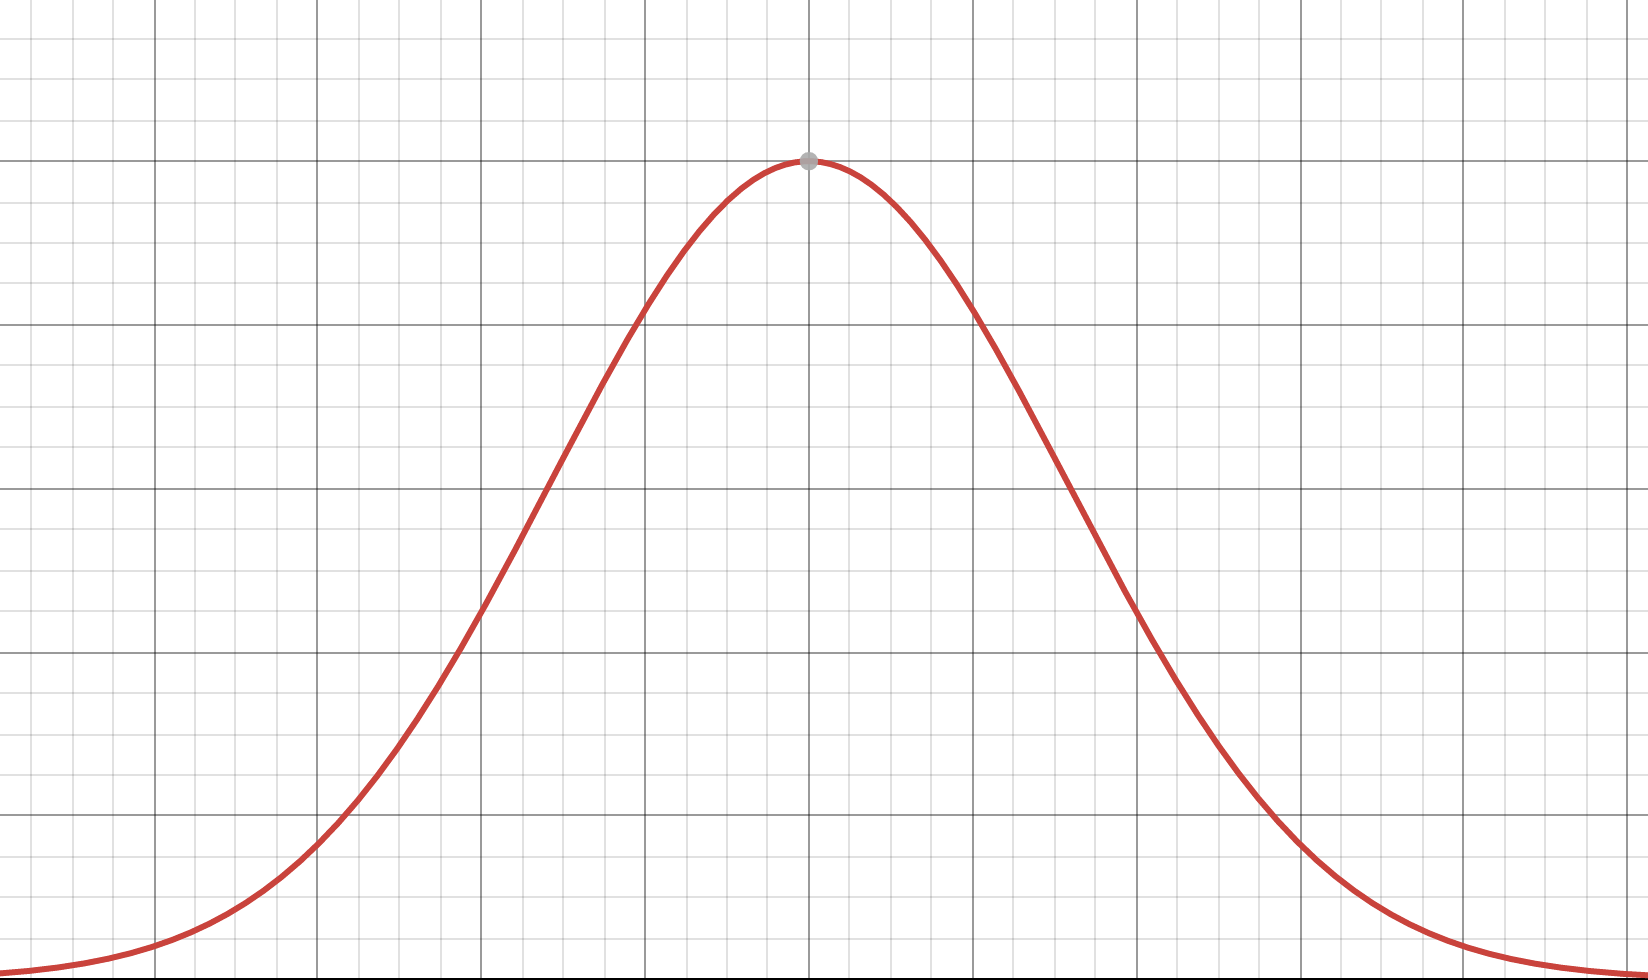
\includegraphics [scale = 0.2] {BellCurve} \hspace{1.5 in} 
\includegraphics [scale = 0.2] {BellCurveMod}
\\*The second professor adds his salary to the number, mods it by L, then gives it to then next professor until all n professors have added their salary and modded the result. After the first professor receives the number from the nth professor, he subtracts his random number then mods the result by L to get the total salary of all the professors. Dividing by the amount of professors in the room n results in the average salary of all the professors in the room without any information leakage.
\vspace{0.5cm}
\\*\centerline{Total Salary $<$ 1 Trillion\hspace{0.75in} 1 Trillion $<$ L\hspace{0.75in} 0 $<$ Random Number, R0 $<$ L}
\smallskip
\\*\centerline{Professor One Adds Salary to R then Mods by L:} 
\\*\centerline{(S$_1$ + R$_0$) mod L}
\smallskip
\\*\centerline{Modding Ensures Uniform Distribution Resulting in Another Random Number:}
\\*\centerline{[(S$_1$+R$_0$) mod L] = R$_1$}
\smallskip
\\*\centerline{All n Professors Do the Same:}
\\*\centerline{[(S$_2$+R$_1$) mod L] = R$_2$}
\\*\centerline{[(S$_3$+R$_2$) mod L] = R$_3$}
\\*\centerline{. . .}
\\*\centerline{After All n Professors Added their Salary and Modded the Result:}
\\*\centerline{R$_n$ = (Total Salary of Professors + R$_0$) mod L}
\\*\centerline{Total Salary of Professors = (R$_n$ - R$_0$) mod L}
\smallskip
\\*\centerline{Divide the Total Salary by n to get the Average Value:}
\\*\centerline{Total Salary / n = Average Salary}
\medskip
\item\textbf{Collaborated with Ivan Lin}
\smallskip
\\*\uline{My Explanation}
\\* Similar to part a, the professors start by agreeing on a number L that has a value much larger than one trillion. The first professor picks a random number R$_1$ between 0 and L-1 inclusive. However, instead of the first professor adding his salary to the random number, he splits it into n smaller random numbers that add up to the initial random number r$_1$ to r$_n$. He then randomly picks a number between r$_1$ to r$_n$ inclusive before distributing the rest to the other professors. After the other n-1 professors repeat the same process, each professor should have two random numbers: the random number they chose between 0 and L -1 (R$_n$) and the sum of all the random pieces they were given ($\sum_{i=1}^{n} r_{i}$). 
The first professor then adds either R$_1$ or $\sum_{i=1}^{n} r_{i}$ to his salary (for the sake of this explanation, I'll say he uses R$_1$)
\smallskip
\\*\centerline{Current Total = S$_1$ + R$_1$}
\smallskip 
\\*Rather than telling the professor next to him, the first professor says his number aloud for all professors to hear. The next professor volunteers and then adds his salary (S$_2$) plus his random number (R$_2$) to the current total.
\\*\centerline{Current Total = S$_1$ + R$_1$ + S$_2$ + R$_2$}
\smallskip
\\*The remaining professors do the same resulting in:
\smallskip
\\*\centerline{Total = Total Professor Salaries ($\sum_{i=1}^{n} S_{i}$) + Total Random Numbers ($\sum_{i=1}^{n} R_{i}$)}
\smallskip
\\*To figure out the total professor salaries, the professors all subtract the sum of their random pieces ($\sum_{i=1}^{n} r_{i}$)
\\*\centerline{$\sum_{i=1}^{n} R_{i}$ = $\sum_{i=1}^{n}\sum_{i=1}^{n} r_{i}$}
\smallskip
\\*\centerline{Total Professor Salaries ($\sum_{i=1}^{n} S_{i}$) = Total - Total Random Pieces ($\sum_{i=1}^{n}\sum_{i=1}^{n} r_{i}$)}
\smallskip
\\*To find the average of their salaries, the professors divide their total by n.
\smallskip
\\*\centerline{Average Professor Salary = Total Professor Salaries / n}
\newpage
\uline{Ivan's Explanation}
Given $n$ professors and a huge number $L$.\newline

Each professor randomly chooses a random number $R$ uniformly distributed from 0 to $L$.\newline

Each professor then randomly distributes $R$ into $n$ components (divided randomly, not evenly) that add up to $N$, where each component is represented by $r$.\newline

Every professor receives one of these components, and this is true for each professor, so each professor eventually has their salary, $S$, and the sum of the salary components from other professors, $\sum_{i=1}^{n} r_i$.\newline

The professors each take $S+\sum_{i=1}^{n} r_i$ (the sum of their salary and the sum of the components they received) together. \newline

Each takes that total modulo $L$ (which obfuscates the expected value), and add them all together with that of other professors.\newline

$\sum_{i=1}^{n} [(S_i + \sum_{j=1}^{n} r_{i,j})\%L] = \sum_{i=1}^{n} [(S_i + R_i)\%L$].\newline

The total is equal to the sum of all salaries and all individual components, which is also equal to the sum of all salaries and all the originally chosen random numbers.\newline

Each professor than subtracts their original random number, $R_i$, from the total.\newline

\noindent\rule{10cm}{0.4pt}\newline

\textbf{Note} Alternatively, each professor add $(S + R)\%L$ (their salary and their original random number) to the total. Each professor then subtracts $\sum_{i=1}^{n} r_i$ (the sum of the components they receive) from the sum total.\newline

\noindent\rule{10cm}{0.4pt}\newline

Regardless of the method, $\sum_{i=1}^n R_i = \sum_{i=1}^n \sum_{j=1}^n r_{i,j}$. The total sum of the random numbers are equal to that of the random components. However, each individual professor's random number $R$ and component sum $\sum_{i=1}^n r_i$ are different, so it is impossible to discern each professor's individual salary.\newline

Once the random numbers have been subtracted and the difference has been found, the answer should first be taken modulo $L$. The output is then $\sum_{i=1}^n S_i$, which can be divided by $n$ to find the average salary of the professors.
\end{enumerate}

\end{document}